% SECTION ====================================================================================
\vspace{-4pt}
\begin{sectionbox}
\section{Natürliche Suchbäume}
% ============================================================================================
\subsection{Nomenklatur}
\begin{center}
    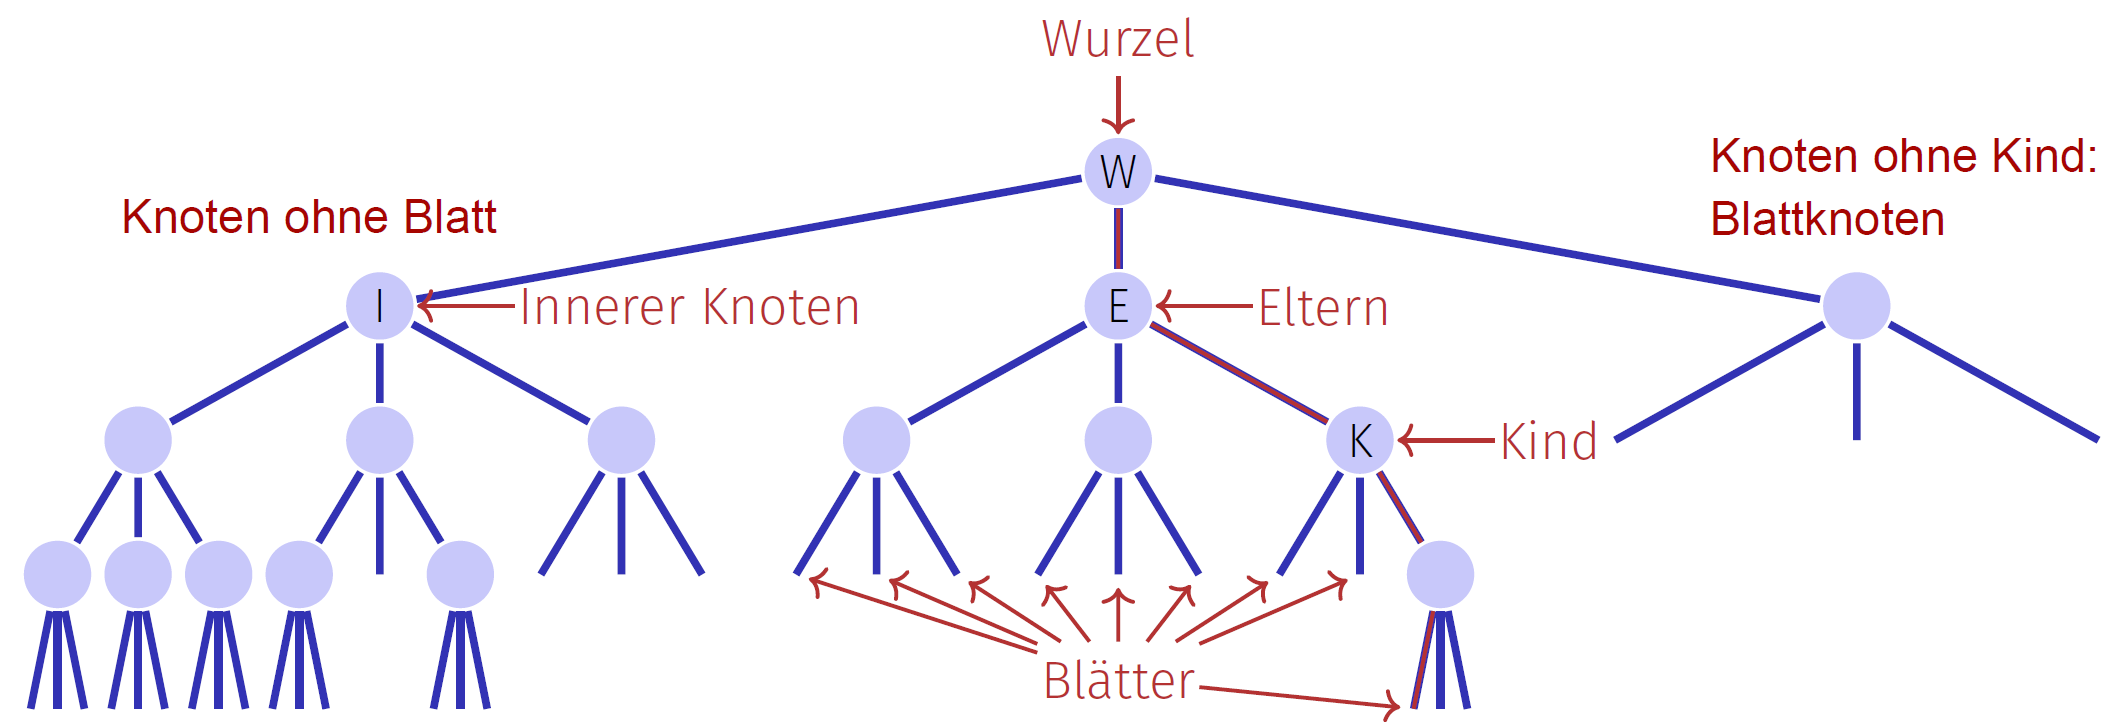
\includegraphics[width = \columnwidth]{../img/BaumNomen.png}
\end{center}
\end{sectionbox}
\vspace{-4pt}
\begin{sectionbox}
  \subsection{Binäre Suchbäume}\smallskip
  Binärer Baum (nur zwei Nachfolgerknoten) mit Eigenschaften:\par
  \begin{itemize}
      \item Jeder Knoten v speichert einen Schlüssel
      \item Schlüssel im linken Teilbaum v.left kleiner als v.key
      \item Schlüssel im rechten Teilbaum v.right grösser als v.key
  \end{itemize}\vspace{7px}
  
  \subsubsection{Höhe eines Baumes}\smallskip
  $h(r)=\left\{\begin{array}{ll}0 & \text { falls } r=\text { null } \\ 1+\max \{h(r \cdot \operatorname{left}), h(r \cdot \text { right })\} & \text { sonst. }\end{array}\right.$\par\smallskip
  Die Laufzeit der Suche ist somit im schlechtesten Fall $\mathcal{O}(h(T))$.\par\smallskip
  \end{sectionbox}
  \vspace{-4pt}
  \begin{sectionbox}
  \subsubsection{Operationen}\smallskip
  
  \textbf{Knoten entfernen}\par
  Mögliche Situationen: Knoten hat keine Kinder, Knoten hat ein Kind oder Knoten $v$ hat zwei Kinder.
  Im letzten Fall: Der kleinste Schlüssel im rechten Teilbaum $v.right$ ist der symmetrische Nachfolger von $v$ $\rightarrow$ ersetze $v$ durch seinen symmetrischen Nachfolger.
  \par Auch möglich: ersetze $v$ durch seinen symmetrischen Vorgänger
  \par Implementation: der Teufel steckt im Detail!
  \end{sectionbox}
  \vspace{-4pt}
  \begin{sectionbox}
  \textit{Grafik zu dem symmetrischen Vorgänger (links) oder Nachfolger (rechts)}\par
  \begin{center}
  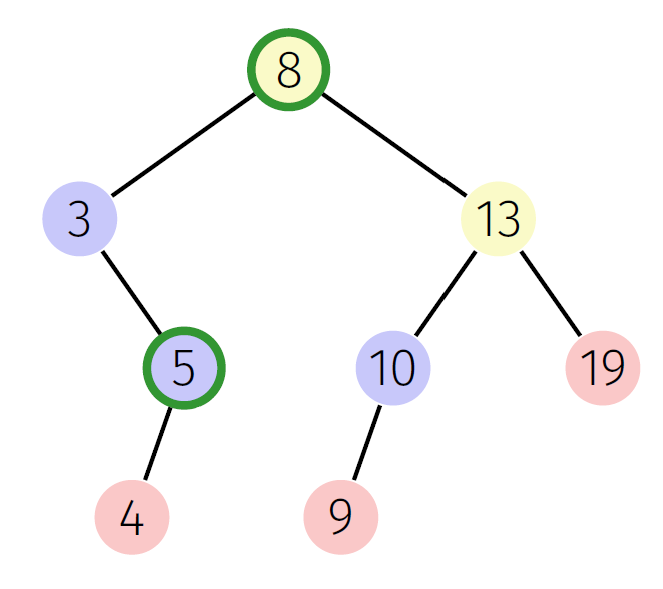
\includegraphics[width = 0.4\columnwidth]{../img/symVorg.png}
  \tab 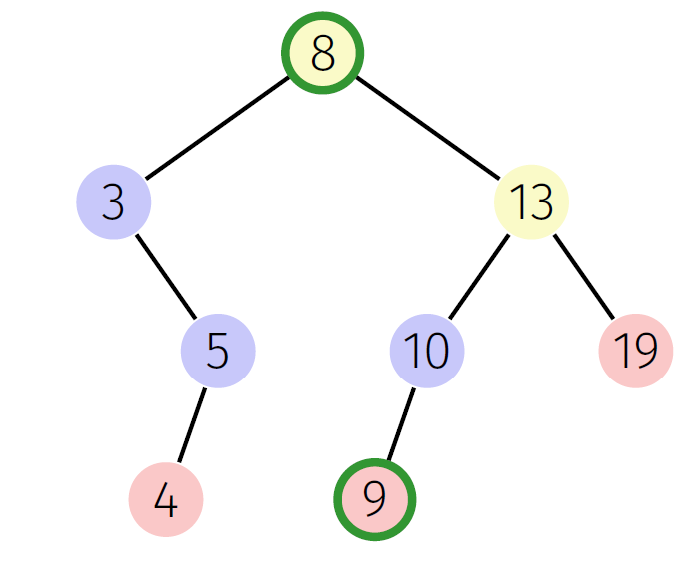
\includegraphics[width = 0.4\columnwidth]{../img/symNachf.png}    
  \end{center}
  \end{sectionbox}
  \vspace{-4pt}
  \begin{sectionbox}
  \subsection{Traversierungsarten}\smallskip
  \begin{greenbox}
  \begin{itemize}
      \item \textbf{Hauptreihenfolge} (preorder):
      \par $v$, dann $T_{left}(v)$, dann $T_{right}(v)$.
      \item \textbf{Nebenreihenfolge} (postorder):
      \par $T_{left}(v)$, dann $T_{right}(v)$, dann $v$.
      \item \textbf{Symmetrische Reihenfolge} (inorder):
      \par $T_{left}(v)$, dann $v$, dann $T_{right}(v)$.
  \end{itemize}
  \end{greenbox}\smallskip
  
  \textit{Beispiel}\par
  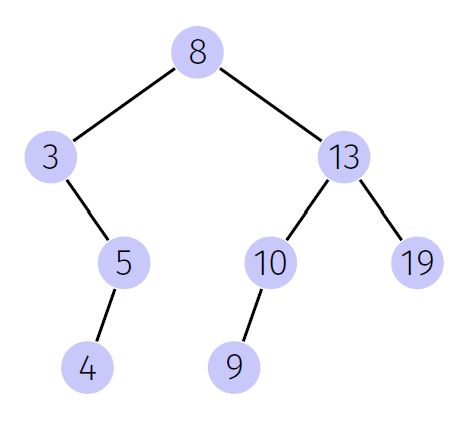
\includegraphics[width = 0.4\columnwidth]{../img/BspBST.png}
  \smallskip
  \begin{itemize}
      \item \textbf{Hauptreihenfolge} (preorder):
      \par 8, 3, 5, 4, 13, 10, 9, 19
      \item \textbf{Nebenreihenfolge} (postorder):
      \par 4, 5, 3, 9, 10, 19, 13, 8
      \item \textbf{Symmetrische Reihenfolge} (inorder):
      \par 3, 4, 5, 8, 9, 10, 13, 19
  \end{itemize}
\end{sectionbox}


\subsection{C++ - Implementation}\smallskip
\subsubsection{Tree}\smallskip
\begin{lstlisting}[language=C++]
class BST {
  Node* root;
public:
  BST();
  bool contains(int key) const;
  bool insert(int key);
  bool remove(int key);
  void print_preorder(std::ostream& out) const;
  void clear();
  ~BST();
};

// Constructor, creates an empty binary search tree
BST::BST(): root(nullptr) {}

// Returns true iff the BST contains the given key.
bool BST::contains(int key) const {
  return root == nullptr ? false : root->contains(key);
}
  
// Returns true iff the given key was inserted into the BST.
bool BST::insert(int key) {
  if (root == nullptr) {
    root = new Node(key);
    return true;
  } else {
    return root->insert(key);
  }
}
  
// Returns true iff the given key was removed from the BST.
bool BST::remove(int key) {
  if (root == nullptr) {
    return false;
  } else if (root->key == key) {
    root = Node::symmetric_successor(root);
    return true;
  } else {
    return root->remove(key);
  }
}
  
// Prints the preorder-traversal of the BST to out.
void BST::print_preorder(std::ostream& out) const {
  if (root != nullptr) {
    root->print_preorder(out);
    out << '\n';
  }
}

// Clears the BST, i.e. resets it to empty.
void BST::clear() {
  delete root;
  root = nullptr;
}

// Deconstructor
BST::~BST() {
  clear();
}
\end{lstlisting}



\subsubsection{Node}\smallskip
\begin{lstlisting}[language=C++]
struct Node {
  int key;     // Key, i.e. value stored in this node
  Node* left;  // Left child, i.e. root of left subtree
  Node* right; // Right child, i.e. root of right subtree
  
  Node(int key, Node* left, Node* right);
  
  bool contains(int search_key) const;
  bool insert(int new_key);
  bool remove(int remove_key);
  void print_preorder(std::ostream& out) const;
  static Node* symmetric_successor(Node* root);
  ~Node();
};

// Node constructor
Node::Node(int key, Node* left, Node* right): 
        key(key), left(left), right(right) {}

// POST: Returns true iff the tree contains search_key.
bool Node::contains(int search_key) const {
  const Node* curr = this;
  
  while (curr != nullptr) {
    if (curr->key == search_key) {
      return true;
    } else if (search_key < curr->key) {
      curr = curr->left;
    } else {
      assert(search_key > curr->key);
      curr = curr->right;
    }
  }
  return false;
}

// POST: Inserts new_key into the tree, if not already 
//  present. Returns true iff new_key was inserted.
//  Maintains the binary search-tree invariant.
bool Node::insert(int new_key) {
  Node* curr = this;
  
  while (curr->key != new_key) {
    if (new_key < curr->key) {
      if (curr->left == nullptr) {
        curr->left = new Node(new_key);
        return true;
      } else {
        curr = curr->left;
      }
    } else {
      assert(new_key > curr->key);
      if (curr->right == nullptr) {
        curr->right = new Node(new_key);
        return true;
      } else {
        curr = curr->right;
      }
    }
  }
  return false;
}

// PRE:  this->key != remove_key, i.e. remove_key may be 
//  contained in this node's subtrees, but not in this node 
//  directly.
// POST: If this tree contained remove_key, then the corre-
//  sponding node was removed, replaced by its symmetric 
//  successor, and true is returned. Otherwise, nothing was 
//  changed, and false is returned. 
//  Maintains the binary search-tree invariant.
bool Node::remove(int remove_key) {
  assert(this->key != remove_key);
  
  // curr descends down the tree, while we look for the a 
  // node with remove_key.
  // curr's key itself is always different from remove_key.
  Node* curr = this;
  Node* remove_node = nullptr;
  
  while (curr != nullptr && remove_node == nullptr) {
    if (
      curr->left != nullptr&& curr->left->key == remove_key){
      // curr's left child holds remove_key, and is replaced 
      // with its symmetric successor.
      remove_node = curr->left;
      curr->left = symmetric_successor(curr->left);
    } else if (
      curr->right != nullptr && 
      curr->right->key == remove_key) {
      // Analogously, for curr's right child
      remove_node = curr->right;
      curr->right = symmetric_successor(curr->right);
    } else if (remove_key < curr->key) {
      // Descend left
      curr = curr->left;
    } else {
      // Descend right
      assert(remove_key > curr->key);
      curr = curr->right;
    }
  }
  
  if (remove_node != nullptr) {
    // To prevent memory leaks, the removed node is freed
    remove_node->left = nullptr;
    remove_node->right = nullptr;
    delete remove_node;
    return true;
  } else {
    return false;
  }
}

// POST: Prints the tree's keys in preorder traversal to out.
void Node::print_preorder(std::ostream& out) const {
  out << key << ' ';
  if (left != nullptr) left->print_preorder(out);
  if (right != nullptr) right->print_preorder(out);
}

// PRE:  root != nullptr 
// POST: Returns the symmetric successor of the given root
//  node. If the symmetric successor is not a direct child of 
//  the given root, then the symmetric successor is also 
//  removed from its context, i.e. from the subtree of root 
//  where the symmetric successor was found.
Node* Node::symmetric_successor(Node* root) {
  assert(root != nullptr);
  
  // If there's at most one child node, it must be the 
  // symmetric successor, and we're done right away.
  if (root->left == nullptr) return root->right;
  if (root->right == nullptr) return root->left;

  // Otherwise, the symmetric successor must be the left-most 
  // element of root's right subtree. We use curr to descend 
  // down the tree, and parent will have parent->left == curr 
  // (if parent != nullptr). parent needed for removing the 
  // eventually found symmetric successor from its context.
  Node* curr = root->right;
  Node* parent = nullptr;
  
  // Descend leftwards. After the loop, curr is the symmetric 
  // successor.
  while (curr->left != nullptr) {
    parent = curr;
    curr = curr->left;
  }

  // Remove the symmetric successor from its context, if 
  // necessary.
  if (parent != nullptr) {
    parent->left = curr->right;
    curr->right = root->right;
  }

  curr->left = root->left;
  return curr;
}

// Deconstructor. All transitive children are recursively 
// deleted. 
Node::~Node() {
  delete left;
  delete right;
}
\end{lstlisting}
